
\documentclass[camera-ready,twocolumn,10pt]{IEEEtran}
\usepackage{usenix,epsfig,endnotes}
\usepackage{color}
\usepackage{amssymb}
\usepackage{algorithm}
\usepackage[noend]{algorithmic}
\usepackage{graphicx,subfigure}
\DeclareGraphicsExtensions{.eps,.ps,.eps.gz,.ps.gz,.eps.Z}
\usepackage{stfloats}
\usepackage{float}
\usepackage{caption}
\begin{document}

%don't want date printed
\date{}

%make title bold and 14 pt font (Latex default is non-bold, 16 pt)
\title{\Large \bf START: Status and Region Aware Taxi Mobility Model for Urban Vehicular Networks}

%for single author (just remove % characters)
\author{
{\rm Haiquan Wang}\\
{\rm Wenjing Yang}\\
{\rm Jingtao Zhang}\\
{\rm Jiejie Zhao}\\
School of Software, Beihang University, Beijing, P.R.China\\
Beijing Key Laboratory of Network Technology, Beijing, P.R.China\\
\and
{\rm Yu Wang\thanks{
 This research has been partially supported by the US National Science Foundation (NSF) under Grant No. CNS-1319915 and CNS-1343355, the National Natural Science Foundation of China (NSFC) under Grant No.61300173 and No. 61170295, the Project of Aeronautical Science Foundation of China under Grant No.2013ZC51026 and No.2011ZC51024, the Fundamental Research Funds for the Central Universities under Grant No. YWF-12-LXGY-001, and the State Key Laboratory Software Development Environment and Network Information and Computing Center of Beihang University.}}\\
Department of Computer Science, University of North Carolina at Charlotte, NC, USA\\
% copy the following lines to add more authors
% \and
% {\rm Name}\\
%Name Institution
} % end author

\maketitle


\subsection*{Abstract}
Using a realistic mobility model will enhance the validity of simulations. However, the difficulty lies in discovering laws from large amounts of data and applying those rules. Researchers have been working on mobility model extracting from real data set, whereas the taxi behavior differences between different taxi statuses have been ignored in previous works.
Based on the the experience in daily life, two assumptions related to the taxi status, one is the behavior of taxi will be influenced by the statuses and the other one is the macroscopic movement is related with different geographic feathers in corresponding status, are introduced and estimated by the real data. Based on the two assumptions, a novel taxi mobility model START is proposed with respect to taxi status. The simulation results illustrate that proposed mobility model has a good approximation with reality in trace samples, distribution of nodes and the contact characteristics.

\subsection*{keyword}
mobility model, taxi status,region recognition

\section{Introduction}
\label{section_introduction}

In vehicle ad hoc networks (VANETs) \cite{4068700}, realistic mobility model is an important way to improve route planning, control traffic situations, or solve the vehicle-to-vehicle communication problems. However, mobility models might influence simulation performance, since mobility model defines the nodal mobility pattern including speed and direction. However, large amount of data are difficult to be utilized directly. It is necessary to work on realistic mobility models. Some researchers \cite{KimKotz-99,HuangZhu-88} modeled the vehicular mobility, extracting different feathers from real data sets. Nevertheless, taxi status is ignored in the previous works.

In this work, a STatus and Region Aware Taxi mobility model, STRAT, is proposed based on the real taxi GPS data. Two assumptions are introduced in section \ref{section_assumptions_anlysis}. We assume that the taxi behavior and geographic features are related with different status. They are verified to be reasonable by the statistical analysis of the data set.
START is modeled based on these assumptions. In the macro scope, instead of simply dividing the area into coarse-grain regions, we classified the area into two set of regions according to the passenger loading or droping event density. When a taxi take a passenger, the current region will be selected from the region set of load-event and the destination region, where the drop-event happens, will be selected from the region set of drop-event. We investigate the relationship between load-event regions and drop-event regions. Paths from the sources to destinations will be found by Dijkstra algorithm. In detailed view, the \emph{speed} for the two taxi statuses are discussed respectively.
Simulations are carried out to compare the similarity of node trace characteristics and contact characteristics. The results show that our mobility model has a good approximation with the real scenario in trace samples, distribution of nodes and the contact characteristics.

The rest of our paper is organized as follows: %%Section \ref{section_related_works} provides an overview of related works on mobility models.
 Section \ref{section_assumptions_anlysis} proposes two assumptions which are further validated by statistical results of real data. Section \ref{section_modeling} presents the modeling process. Simulation results are demonstrated in Section \ref{section_model_varification}. Finally, Section \ref{section_conclusion} concludes this paper.




%%\section{Related Works}
\label{section_related_works}

For the free space scenario, the random way point (RWP)\cite{broch1998performance} movement model is the most commonly used. The movement model identified a pause time, speed range from zero to the maximum, and movement area where the model select a random destination. Amit Kumar Saha, el at. \cite{SahaJohnson-91} found that RWP in many cases the Random Waypoint mobility model is a good approximation of the vehicular mobility model based on real street maps.
The constrained mobility models show closer relevance to the realistic. Some models \cite{HuangZhu-88,SahaJohnson-91,MartinezCano-87,ChoffnesBustamante-93} take the geographic structure into consideration. 

In this section,  we sum up the researches on mobility models.Mobility model can be classified into free space and constrained models\cite{LuChen-104,AhmedKarmakar-106} based on the degree of randomness.
Random walk, Random Waypoint and Random Direction mobility model are three classical free style mobility models. Those models defined simple mobility patterns, which is good for us to create mobility models and analysis. But they also have notable disadvantages, e.g., they  are out of reality, because too many factors are ignored. 

In order to increase the degree of reality, mobility models are constrained or relayed in many respects. Some researchers build models based on geographic models. Manhattan models \cite{FBaimanhattan} are a typical models which models the city as a Manhattan style grid, with a uniform block size across the simulation area, while all streets are two-way with a lane in each direction which constrained car movements \cite{MartinezCano-87}, and nodes can move straight forward or turn direction at a cross road.
Other models import the map information into mobility models. In 2004, Saha, A.K \cite{SahaJohnson-91} model the vehicle networks based on the real map. It compared with the RWP models, a frequently used model in vehicular networks, to find out the difference between the RWP and real traces. In 2005, literature \cite{ChoffnesBustamante-93} proposed a comprehensive models on wireless vehicular networks and transportation. This paper simplifies the real map to estimate the network performance in ad hoc and proposes the mobility model STRAW. Besides, some other mobility focus on the microscopic characteristics of mobility, they introduce the transportation features into mobility, such as the traffic lights and accretion on some road segments. The information of the geography can improve the reality. In 2007, Atulya Mahajan, et al. \cite{MahajanPotnis-102} accounted for the street layout, traffic rules, multi-lane roads, acceleration-deceleration, and radio frequent (RF) attenuation due to obstacles, and further evaluated the synthetic maps by comparing with real maps. In 2008, David R. Choffnes, et al.\cite{ChoffnesBustamante-93} developed their movement model based on a realistic vehicular traffic model on road defined by real street map data. but too many microscopic detail can not be applied to scenarios with large scale nodes.

In recent years, vehicular sensors or handheld devices spread rapidly, that makes it possible to collect and analyze the real traces of large amount of nodes and helps us to improve the traffic and network macroscopically.
In 2010 and 2012, Huang H, et al. \cite{HuangZhu-88} proposed mobility models based on taxi trace data in Shanghai, China. They designed three parameters, i.e., turn probability, road section speed and travel pattern, which can be estimated by analyzing the data statistically. But it is complicated to re-implement this model, for the model is strongly related to the map they simplified from the real map.
To the best of our knowledge, our work is original to develop mobility models by investigating taxi behavior, time and geographic feathers of different statuses.


\section{Assumptions and Statical analysis of Taxi Trace}
\label{section_assumptions_anlysis}

In this section, we mainly focus on statistical analysis on the speed and duration characteristics on the data set.
Firstly, the data set will be introduced in section \ref{section_trace_data}. Then, two assumptions are proposed and validated in the following sections.

\subsection{Trace Dataset: Beijing Taxi Traces}
\label{section_trace_data}

A real-world GPS data set is used for our analysis, which was generated by $12,455$ taxis in Beijing, China within five days from March 3 to March 7, 2011. In the data set, each entry includes a base station ID, company name, taxi ID, timestamp, current location (including longitude and latitude), speed, event, status, et al. Of all the fields, the taxi ID, time stamp, and current location, status and event are used for study. There are five types of events and four types of statuses in the data set, which are summarized in Table~\ref{table_event_detail}. We only focus on the vacant and occupied statuses (and corresponding 
load and drop events) in this paper. Note that GPS traces from taxis have been used recently for inferring human mobility \cite{Ganti} and modeling city-scale traffics \cite{Aslam}. Therefore, we believe that they are also suitable to characterize the contact patterns among vehicles in large-scale urban scenario.

\begin{table}[!h]
\caption{Events and statuses in Beijing taxi traces}\label{table_event_detail}
\centering
\begin{tabular}{l|l}
  \hline
  {\bf Event} & Explanation \\
  \hline
  0 (drop) & a taxi's status changes to vacant.\\
  \hline
  1 (load) & a taxi's status changes to occupied.\\
  \hline
  2 & set up defense.\\
  \hline
  3 & cancel defense.\\
  \hline
  4 & no event happened.\\
  \hline
  \hline
  {\bf Status} & Explanation \\
  \hline
0 (vacant) & a taxi is vacant. \\
    \hline
1 (occupied) & a taxi is occupied. \\
    \hline
2 & a taxi is setting up defense. \\
    \hline
3 & stop running.\\
  \hline
\end{tabular}
\end{table}








\subsection{Assumptions}
\label{section_statistic_analysis}
According to the experience in daily life, the following two assumptions are given:

\begin{itemize}
  \item \textbf{Assumption 1:}The behavior of a taxi will change when its status changes. When a taxi is occupied, its destination is certain, and the speed of occupied status will accelerate relatively. In contrast, when a taxi is vacant, it will slow down or even stop to search for potential passengers along the road. Thus, taxi behavior characteristics, such as speed and the status duration varies consequently.

  \item \textbf{Assumption 2:} The movement behavior of taxis associates with geographic feathers. When taxis is occupied, the destination may be tend to some places, such as the airport. Meanwhile, when taxis are vacant, drives tend to some hot spots where more people want to take a taxi.
      \begin{enumerate}
        \item The destination selection will be influenced by different regions.
        \item events occurs in different regions un-evenly, passenger drop and load events are distinct.
      \end{enumerate}
\end{itemize}




   Therefore, we analysis the speed,duration and passenger load/drop events distribution to estimate our assumptions.


\subsection{Speed analysis}
In this section, average speed and speed distribution for each status are investigated.

The average speed will increase if taxis are occupied. It varies from 25.48 to 27.978 $km/h$ when taxis are occupied, while it ranges from 9.977 to 11.272 $km/h$ when taxis are vacant.



\begin{figure}
\centering
\includegraphics[width=0.4\textwidth]{figures_201103/assumption/speeddis.eps}
\caption{Speed Distribution for vacant and occupied status.}\label{figure_speed_distribution}
\end{figure}

 To further investigate the speed distribution, proportion for every speed section is calculated, in fig.\ref{figure_speed_distribution}. For example, dot(19,0.0245) means $2.45\%$ records fall in the speed range $[19,20)km/h$. Because the proportion for 0km/h reaching up to 20\% is too large compared with the proportion of other speed section, we do not show it in figures.
Fig. \ref{figure_speed_distribution} shows that speed distribution differs for each status. Most speed records are in the speed section $[0,100] km/h$. For vacant status, in the speed section (0,40], it follows a linear distribution. But for occupied status, a peak occurs in the range of $[8,15] km/h$.  Fig. \ref{figure_speed_distribution} also demonstrates that the speed distribution is with strong regularity for each status.




\subsection{Taxi Status Duration}
The duration distribution for each status are shown in Fig.~\ref{figure_duration_for_each_status}. Status duration represents the time length of a taxi staying in a certain status. The red line presents the duration time distribution for vacant status, and the green one is for occupied status. Note that the red line (vacant status) approaches to  one earlier than than the blue line (occupied status). So the value of vacant duration is smaller than the value of occupied duration. This is reasonable since drivers tend to shorten the waiting time to raise their incomes.
\begin{figure}[!h]
\centering
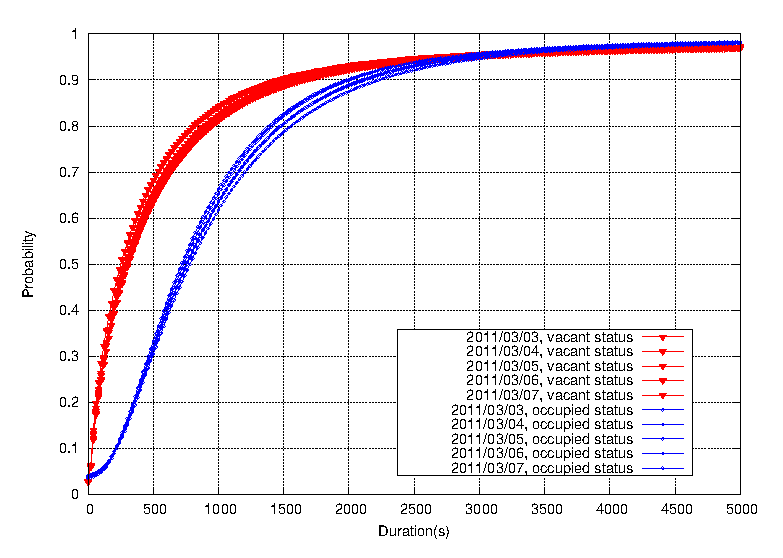
\includegraphics[width=0.38\textwidth]{figures_201103/assumption/durationdis.eps}\\
\caption{Status duration distributions.}\label{figure_duration_for_each_status}
\end{figure}

Overall, the statistical results for both speed and status duration are consistent with \emph{Claim 1}, that is, the behaviors of taxis are similar within each status while differ between the two statuses.


\subsection{Taxi event distribution}
\label{section_taxi_denstiy_distribution}

To validate $assumption 2$, we quantitatively analyze vehicles density in one hour. By dividing the whole network into $100*100$ grids, taxi density distributions for event 0, 1 are computed in each cell.

\begin{figure*}
\centering
\subfigure[$on-event,7:00-8:00$]{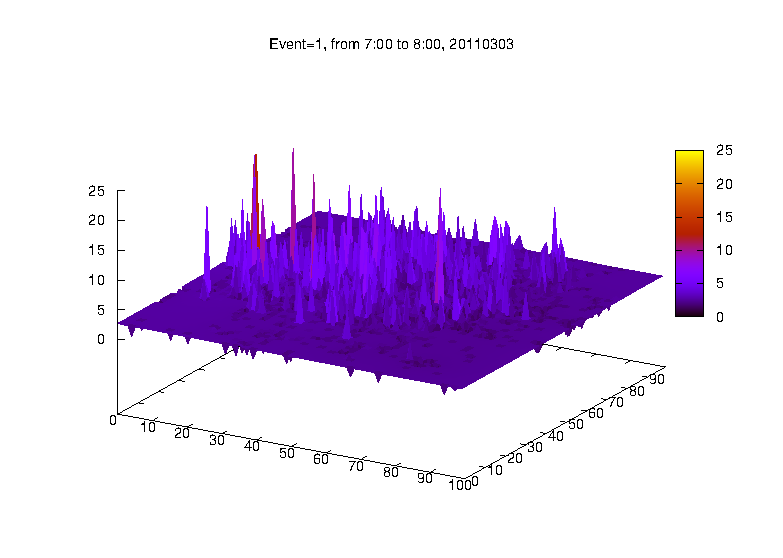
\includegraphics[width=0.3\textwidth]{figures_201103/events_dis/Event=1_7_8_20110303.eps}}
\subfigure[$on-event,12:00-13:00$]{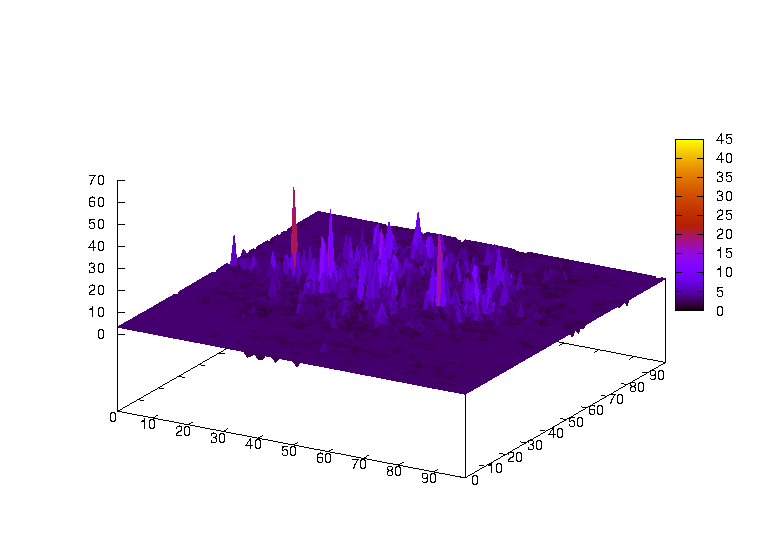
\includegraphics[width=0.3\textwidth]{figures_201103/events_dis/Event=1_12_13_20110303.eps}}
\subfigure[$on-event,17:00-18:00$]{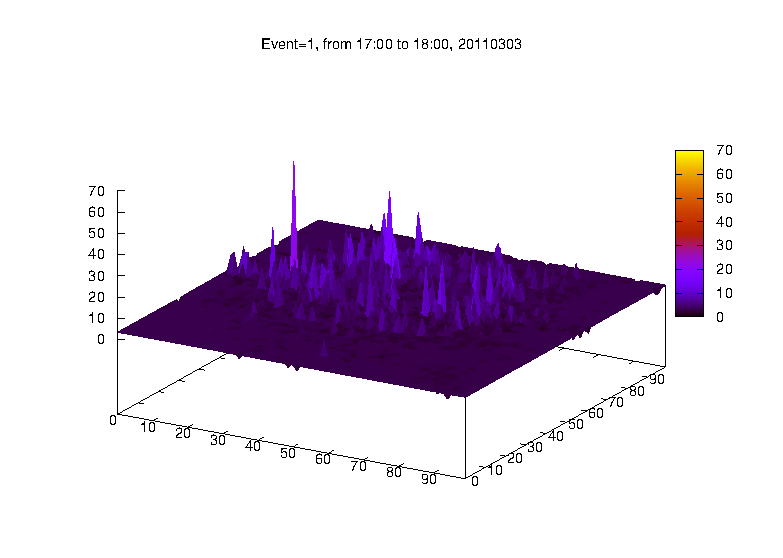
\includegraphics[width=0.3\textwidth]{figures_201103/events_dis/Event=1_17_18_20110303.eps}}
\subfigure[$off-event,7:00-8:00$]{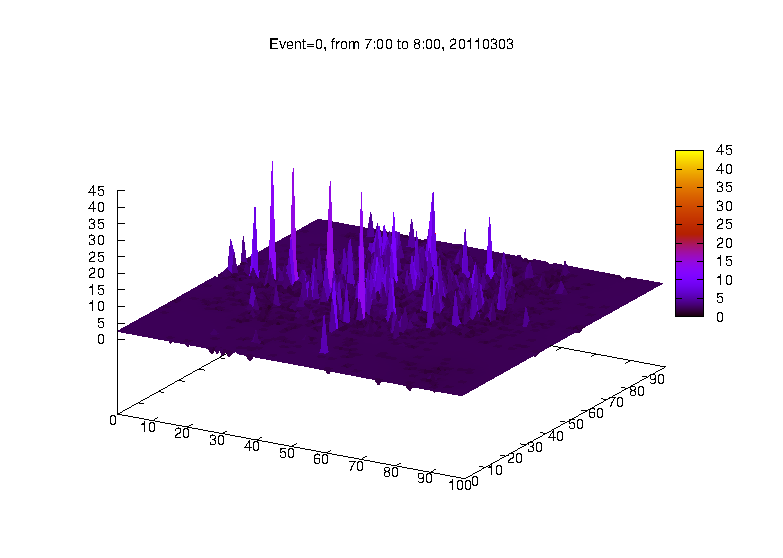
\includegraphics[width=0.3\textwidth]{figures_201103/events_dis/Event=0_7_8_20110303.eps}}
\subfigure[$off-event,12:00-13:00$]{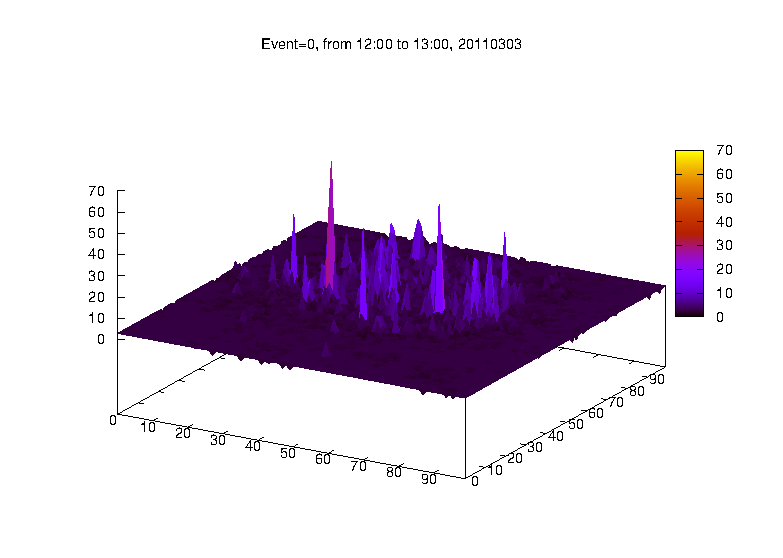
\includegraphics[width=0.3\textwidth]{figures_201103/events_dis/Event=0_12_13_20110303.eps}}
\subfigure[$off-event,17:00-18:00$]{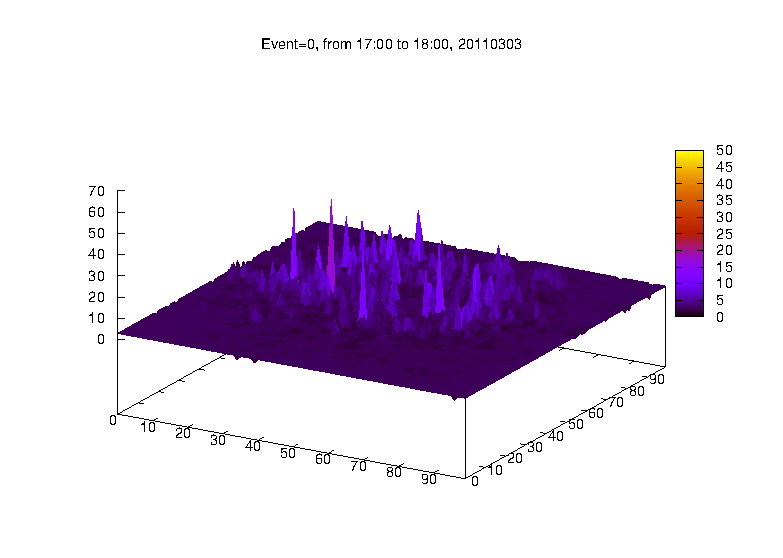
\includegraphics[width=0.3\textwidth]{figures_201103/events_dis/Event=0_17_18_20110303.eps}}
\caption[c]{Taxi density for on-event and off-event in one hour}\label{figure_taxi_density_for_one_hour}
\end{figure*}

Figure.\ref{figure_taxi_density_for_one_hour} shows the on/off events distribution in three time sections. In the morning, people begin to get out. so the on-event distribute is more even than that of off-event. this phenomenon may be caused by the on-event spots are mainly at the homes of the citizens, while the off-event spots tend to gather together at workplaces, railway stations or scenic spots. Besides, in the evening, the dispersion of on-event is of lower degree than that of off-event, for people coming home at that time.

The amount of loading passengers in each cell shows geographic feathers:the distribution is uneven, and the difference between on/off-event distributions illustrates the on/off-event regions are different which support the \emph{assumption 2}.


\section{Modeling}
\label{section_modeling}

\subsection{Overview of START}

Movement model defines the mobility pattern of nodes, which can be represented as a collection of path segments, say $Paths:<p_1,p_2,...,p_n>$.  To generate a $p_i$, START takes two steps: destination selection and moving process (from current location to the selected destination).

\textbf{Destination Selection:} In START, the selection of a destination of a node is closely related to not only its current location but also its current status. Dividing the area into regions by the density of passenger load/drop events, respectively. We will show how to dividing the area in the next subsection. Let $\textbf{R}^{load}=\{R_i^{load}\}$ and $\textbf{R}^{drop}=\{R_j^{drop}\}$ denote the set of regions of load and drop events, respectively. We assume that $\bigcup\{R_i^{load}\}=\bigcup\{R_j^{drop}\}$ which is the whole area.  
Then, two transition probability matrixes are calculated: one is the transition probability from a passenger drop region $R_i^{drop}$ to a passenger load region $R_j^{load}$, while the other is the transition probability from a passenger load region $R_i^{load}$ to a passenger drop region $R_j^{drop}$.
If the status of a taxi changes to vacant, its current location locates in a $R_i^{drop}$. Consequently, a destination region in $\textbf{R}^{load}$ will be selected by querying the transition matrix from $\textbf{R}^{drop}$ to $\textbf{R}^{load}$. Then, START will randomly select a map node in the region as the destination. As to the status of a taxi changing to occupied, the destination selection process is similar except for that the transition matrix from $\textbf{R}^{load}$ to $\textbf{R}^{drop}$ is used instead. In summary, during this process, the destination of drop/load location is randomly selected based on the region transition matrix corresponding to the current status.

\textbf{Moving Process:} When the source location (current location) and destination location are given or selected, the next step is to find a path to connect them. To simplify the process, we adopt the Dijkstra algorithm, which will find a shortest path from the source to the destination based on the map. The speed of the path then is assigned to $speed$ based on the current status. Here, the value of $speed$ is drawn from the average speed distribution of corresponding status, which will be introduced in the last subsection of this section.



\subsection{Region Transition Probability}

A travel path of a taxi can be simplified as a multi-hop process, in which a hop indicates an load/drop event happened. Seeing that, we define a \emph{ region transition probability} to figure out the probability of the next hop falling in a certain region $R_j$ from the current region $R_i$. Particularly, when two successive events are different: one load and one drop. Therefore, the region $R_i$ and $R_j$ are recognized by different metrics, that is, drop or load event distribution. For instance, if the taxi is currently occupied, then the next hop event is the drop one. Hence, choosing a target region from a region set obtained based on drop event distribution is more logical.
%%ÿ���ֲ���ͷһ��Ҫ��&���ţ�����\qquad Ϊ��ո�����

Before defining the region transition probability, we first describe our \textbf{region recognition process}.
Firstly, we divide the area into $100\times 100$ small grids, and define them as cells (as shown in the following equation) where $lon$ and $lat$ are relevant longitude and latitude, $len_x$ and $len_y$ are side length of the grid/cell).
\[C_{x,y}::=\{(lon,lat)|x \le \frac{{lon}}{{len_x}} < x + 1,
y \le \frac{{lat}}{{len_y}} < y + 1\}.\]
Then, we consider a region as a union of adjacent cells, as following.
\[R_m:: = \{ C_{x,y}|\exists C_{i,j} \in R_m
\Rightarrow \|x - i\| \le 1,\|y - j\| \le 1\}.\]
The main idea of clustering cells to regions is merging adjacent cells whose event density is larger than an event threshold $\eta$ into a same region.
For drop/load event, this process is conduct respectively. 
Three parameters, threshold $\eta$, Cluster Size and range $t$, are used in this process. 
Cluster Size defines the size of region, i.e., it is a limitation on the size of a region, saying $\|R_i\|\leq ClusterSize$.
We only consider the top $t$ regions, in which event density of each cells are larger than threshold $\eta$.
The overall clustering algorithm is shown as follows. We sort the $100 \times 100$ cells by event density in descending order, 
and begin with the first cell to search its neighbors whether to join the same region or not using breadth traversal. 
After the top t regions are formed, the other cells which do not belong to the top t regions will also be clustered into regions, 
whose size should still be small than Cluster Size. Consequently, every cells will be clustered into regions and the size of each region are not larger than Cluster Size.
By clustering cells into regions, two region sets, \textbf{$R^{load}$} and \textbf{$R^{drop}$}, can be recognized from the data set. As can be seen from Fig. \ref{figure_region_recognizition}, the differences among load region and drop regions for the Beijing taxi data set are clear.
In this figure, every colored block presents a region.In addition, Cluster Size = 200, range t = 200 (range is the same with Cluster Size by coincidence) and threshold $\eta = 121$ are set for load event and $\eta$ equates with 141 for drop event (these are set by the average event density of the top 5000 cells order by its event density).
\begin{figure}[!t]
\centering
\subfigure[drop event regions]{\includegraphics[width=0.23\textwidth]{figures_201103/region/Areas-2011_event0.eps}}
\subfigure[load event regions]{\includegraphics[width=0.23\textwidth]{figures_201103/region/Areas-2011_event1.eps}}
\centering
\caption{Region recognition}\label{figure_region_recognizition}
\end{figure}

\textbf{Calculation of region transition probability}: After clustering cells into regions, the transition probability from $R_i^{load}$ to $R_j^{drop}$ and the one from $R_i^{drop}$ to $R_j^{load}$, donated as $p_{i\rightarrow j}^{load\rightarrow drop}$ and $p_{i\rightarrow j}^{drop\rightarrow load}$, can be caculated. Since both transition probability can be calculated similarly, we only introduce the detailed one of $p_{i\rightarrow j}^{load\rightarrow drop}$.

First, we count all records in $R_i^{load}$ from the data set,  i.e. $REC_i^{load}=\{r~|~r.location\in{R_i^{load} \textit{ and }  r.event=load}\}$. Let $\|REC_i^{load}\|$ be the amount of such records. For record $r \in REC_i^{load}$, the next event and location can be easily obtained from the data set. Thus, we can get the set of such records whose next event is drop and next location is $R_j^{drop}$, i.e., $REC_{i\to j}^{load\to drop}=\{r~|~r.event=load,~r.event_{next}=drop,~r.location_{current}\in R_i^{load}, \textit{ and }  r.location_{next}\in R_j^{drop}\}$. Let $\|REC_{i\to j}^{load\to drop}\|$ be the amount of such records. We can then easily obtain the transition probability from $R_i^{load}$ to $R_j^{drop}$, as follows,
\[p_{i \to j}^{load \to drop} = \frac{\|REC_{i\to j}^{load\to drop}\|}{\|REC_i^{load}\|.}\]


%\begin{equation}\label{transition_matrix}
%  P^{load\to drop} = (p_{i\to j}^{load\to drop})_{m\times n}
%\end{equation}

%\begin{equation}\label{transition_matrix}
%  P^{drop\to load} = (p_{i\to j}^{drop\to load})_{n\times m}
%\end{equation}

%%\begin{equation}\label{equation_taxiset_matrix}
%\textbf{\emph{P^{on\to drop}}}=(p_{i\to j}^{load\to drop})_{m*n}\\
%\textbf{\emph{P^{drop\to load}}}=(p_{i\to j}^{drop\to load})_{n*m}\\
%\end{equatiload}



\subsection{Parameter estimation of speed distribution}
\label{section_speed_modeling}
In this section, we modeling the speed distribution.Because the probability will be influenced by the length of speed range, so we choose the cumulative distribution for modeling. Then we fit the cumulative distribution to get the cumulative probability distribution function, and then take a derivative with it to obtain the speed probability distribution.

Fig.\ref{formular_ccdf_speed} plots the cumulative distribution of speed. From the figure we can get following information:
\begin{itemize}
  \item In the speed range from about 0 to 40 km/h, the distributions show a linear relationship. While after the range, an exponential relationship can be observed.
  \item For vacant status, the distributions are similar. But on March.5 and 6, 2011, the curves show more similarity than on the other days.
  \item For vacant status, the speed distribution differs with each other evenly.
\end{itemize}

 A segmented function is chosen to fit the cumulative distributions and estimated the parameters. Especially, we respectively discuss the distribution for vacant status on workdays and weekend.
The fit formulas are given as formulas \ref{formular_ccdf_speed}.

\begin{equation}\label{formular_ccdf_speed}
\left\{
\begin{array}{ll}
 g(x)=a*x+b & x \in [0,40]\\
 f(x)=1-exp(-c*x-d)& x\in(40,120]\\
\end{array}
\right.
\end{equation}


Fig. \ref{figure_fit_ccdf_speed} also plots the fit results. For vacant status, we discuss the condition for that on workdays and weekend. The blue lines represent the fitting results for the speed range $[0,40] km/h$. And the red lines plot the fitting results for speed range $(40,180] km/h$.
We also fit the cumulative speed distribution for each status, shown as the right bottom in fig.\ref{figure_fit_ccdf_speed}.

\begin{figure}[htbp]
\centering
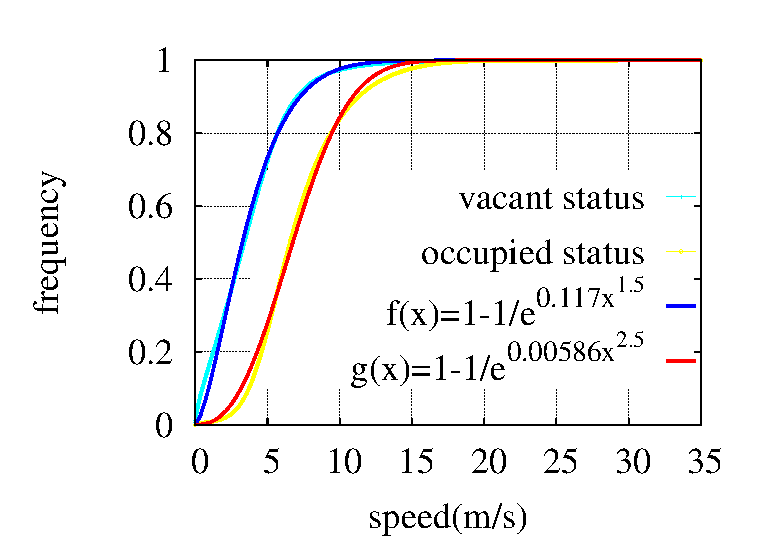
\includegraphics[width=0.4\textwidth]{figures_201103/fit/speedfit.eps}\\
\centering
\caption{The fit result of the cumulative speed distributions.}\label{figure_fit_ccdf_speed}
\end{figure}

The rms of residuals for each fit are as table \ref{table_rms}.The smaller rms of residuals means better fitting. In the table, the values are all less than 0.01, showing good similarity.

\begin{table}[!t]
\caption{The rms of residuals of fitting curves}\label{table_rms}
\centering
\begin{tabular}{l|c}
  \hline
  % after \\: \hline or \cline{col1-col2} \cline{col3-col4} ...
  Categories & rms of residuals  \\
  \hline
  $g_{status=0}^{workday}(x)$[0,40] & 0.00272264\\
  $g_{status=0}^{weekend}(x)$[0,40] & 0.00386982  \\
  $f_{status=0}(x)$(40,120] & 0.00148225\\
  $g(x)_{status=1}$[0,40]& 0.0176819 \\
  $f(x)_{status=1}$(40,120] & 0.00760913\\
  $g(x)_{status=0,1}$[0,40]& 0.0160319\\
  $f(x)_{status=0,1}$[40,120]& 0.00299414\\
  \hline
\end{tabular}
\end{table}



%%\subsection{Status duration distribution modeling}
\label{section_lasting_time_modeling}
Similar to the modeling process of speed, we explore the cumulative distribution of lasting time. Then we fit the cumulative distribution to get the cumulative distribution formular and its estimated parameters.
The fit formulas are given as formulae \ref{formular_ccdf_lasting_time}, and the fitting results are shown as  fig. \ref{figure_fit_ccdf_lasting_time}.
\begin{equation}\label{formular_ccdf_lasting_time}
\begin{array}{ll}
 \phi(x)=1-exp(-e*x)& x\in [0,43200]\\
\end{array}
\end{equation}

\begin{figure}[htbp]
\centering
\includegraphics[width=0.4\textwidth]{figures_201103/fit/duration_fit.eps}\\
\caption{The fit result of the cumulative status duration distributions.}\label{figure_fit_ccdf_lasting_time}
\end{figure}


The fitting result for status 0 is $\phi(x)_0=1-exp(-0.00149701*x)$, and the rms of residuals is 0.0347105. The fitting result for status 1 is $\phi(x)_1=1-exp(-0.000969622 *x)$  and the rms of residuals is 0.0337265.


\begin{figure*}[!t]
\centering
\subfigure[Real Trace]{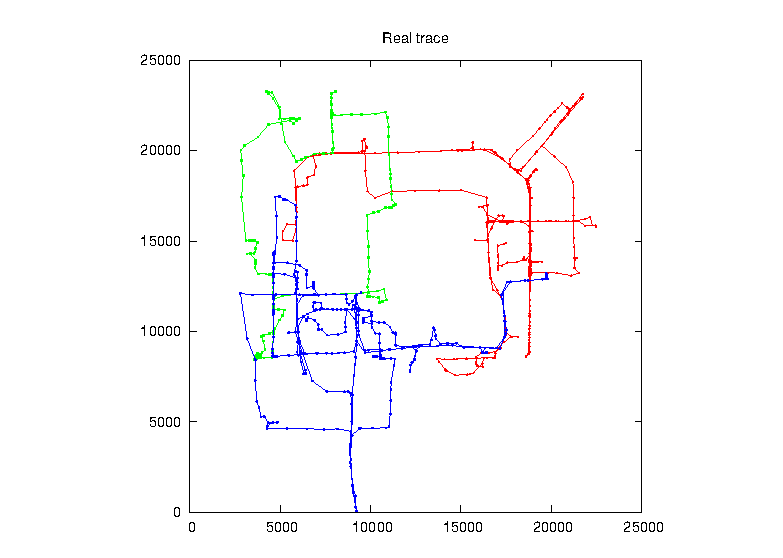
\includegraphics[width=0.24\textwidth]{figures_201103/Evaluation/trace_real.eps}}
\subfigure[START]{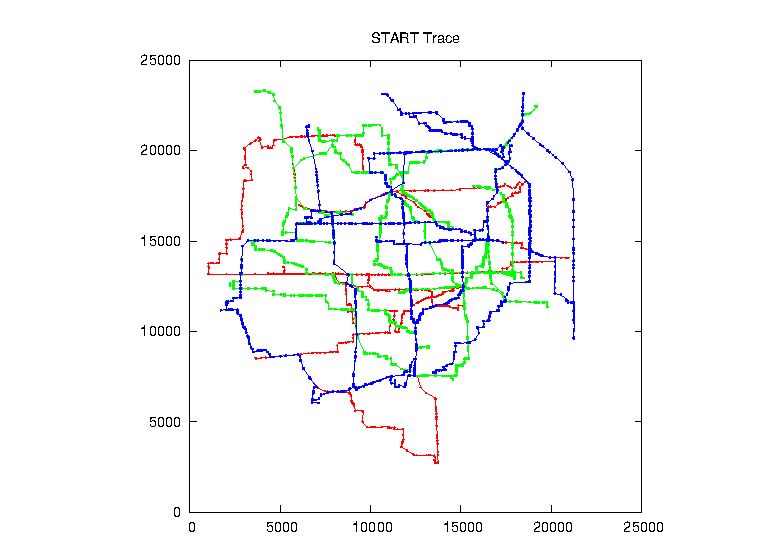
\includegraphics[width=0.24\textwidth]{figures_201103/Evaluation/trace_start.eps}}
\subfigure[SP]{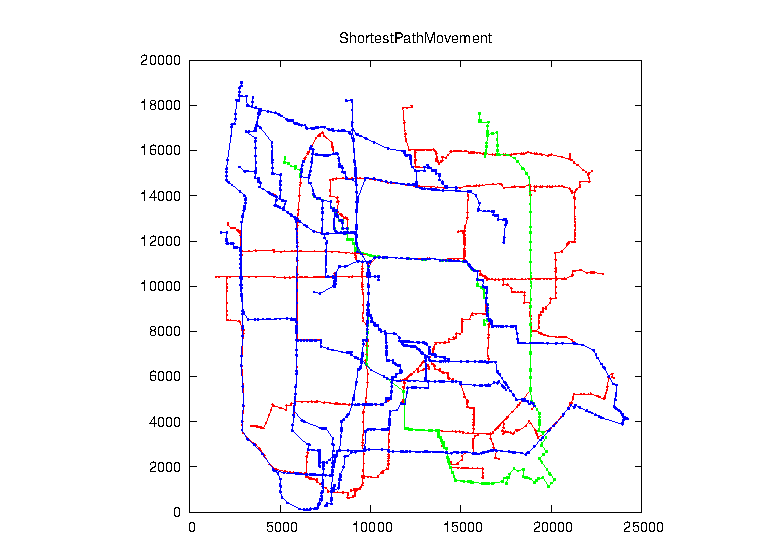
\includegraphics[width=0.24\textwidth]{figures_201103/Evaluation/trace_sp.eps}}
\subfigure[RWP]{\includegraphics[width=0.24\textwidth]{figures_201103/Evaluation/trace_rwp.eps}}
\caption{Trace samples.}\label{figure_tracesample}
\end{figure*}
\begin{figure*}[!t]
\centering
\subfigure[Real Trace]{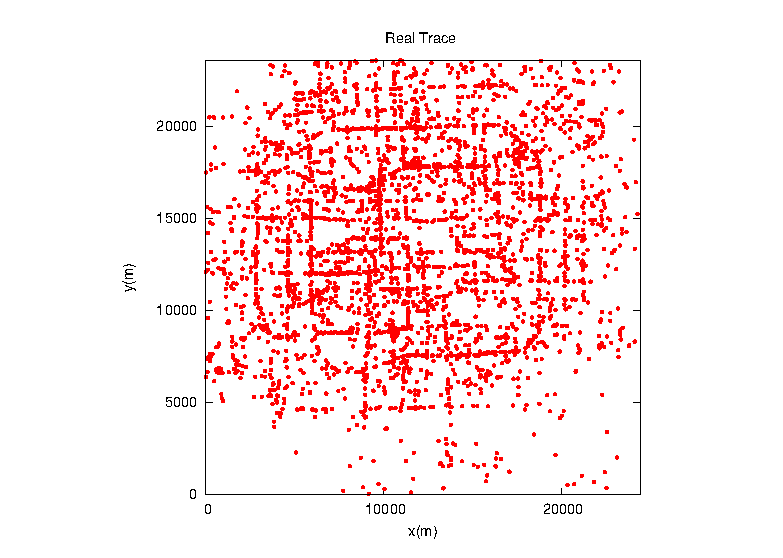
\includegraphics[width=0.24\textwidth]{figures_201103/Evaluation/sample/tracesample.eps}}
\subfigure[START]{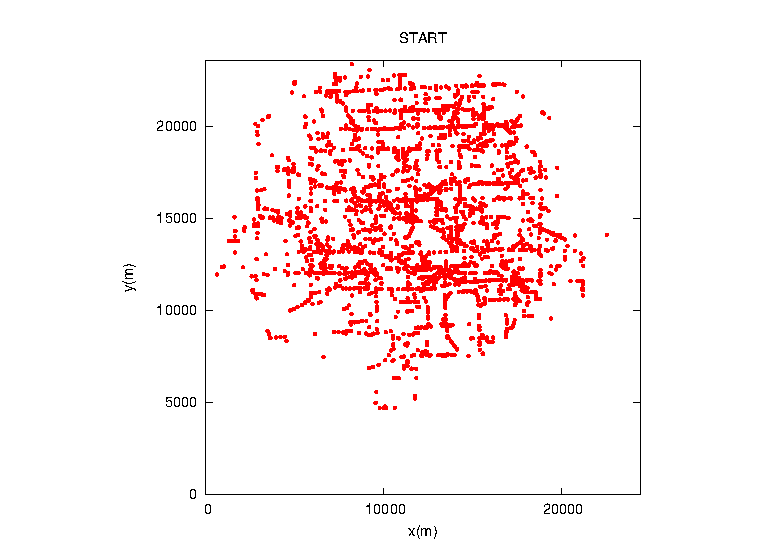
\includegraphics[width=0.24\textwidth]{figures_201103/Evaluation/sample/startsample.eps}}
\subfigure[SP]{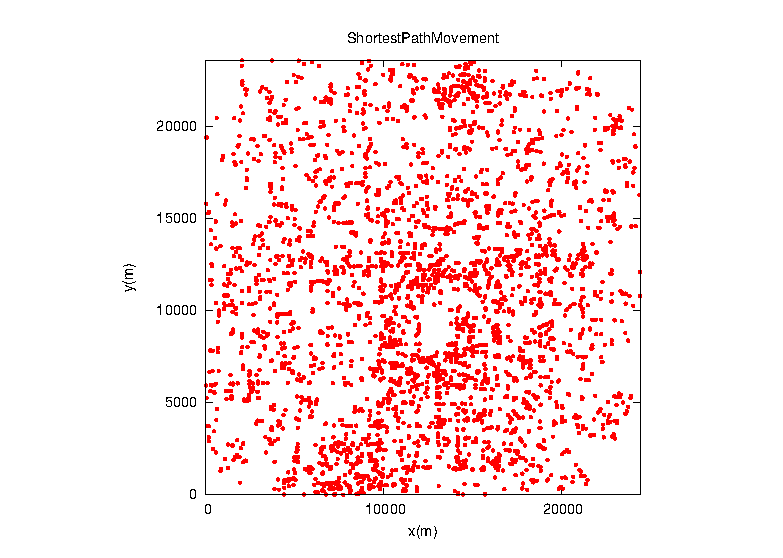
\includegraphics[width=0.24\textwidth]{figures_201103/Evaluation/sample/spsample.eps}}
\subfigure[RWP]{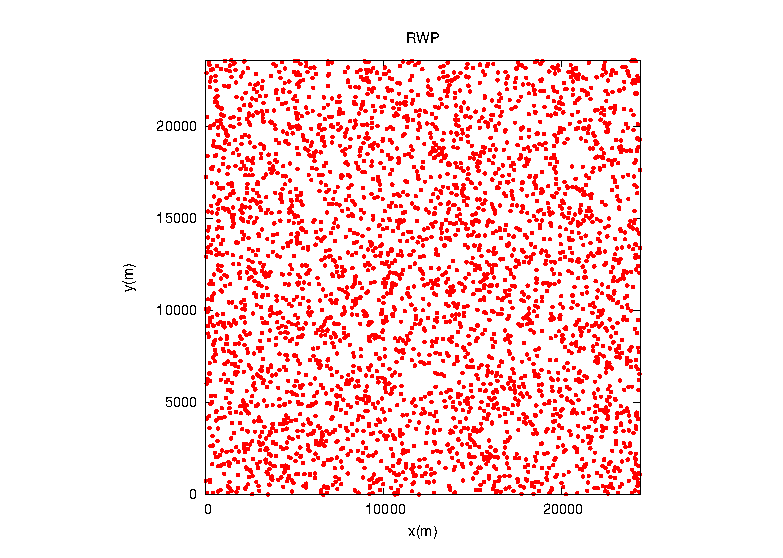
\includegraphics[width=0.24\textwidth]{figures_201103/Evaluation/sample/rwpsample.eps}}
\caption{Trace snapshots.}\label{figure_trace_snapshots}
\end{figure*}

\section{Model Verification}
\label{section_model_varification}
In this section, START mobility model is validated on the aspects of node distribution and contact characteristics compared with existing mobility models and the real traces. We pick two simple mobility models for comparison: one free space - Random Way Point (RWP) model, the other is constrained model, Shortest Path (SP).  SP mobility model is based on the underlying map of Beijing where vehicles move along the map roads by Dijkstra algorithm to random destinations. Both models take no consideration of the node statuses and geographical distributions. All mobility models are implemented on Opportunistic Networking Environment (ONE)\cite{KeranenOtt-155}.

In our simulations, $4,000$ vehicles are deployed in an area of $24,445\times 23,584 m^2$ (a sub-map of the whole area, including fourth ring roads in Beijing). The speed range of RWP and SP need to be configured. To ensure the accuracy, we choose three different speed ranges $[0,44.4]m/s$, $[0,33.3]m/s$ and $[0,22.2]m/s$ (the upper bounds of speed match the speed limits $80$,$120$,$160$ $km/h$. The simulation time is three hours and the warm up time for reports is one hour, so that the nodal movement and positions will not be affected by its initial position. The communication range between vehicles is set to $200m$ for potential contacts.

\subsection{Traces and Node Distributions}

Trace samples and their snapshots from different mobility models are reported in Fig.~\ref{figure_tracesample} and Fig~\ref{figure_trace_snapshots}. Fig.~\ref{figure_tracesample} shows the trace in one day. The traces of the real data and START only cover some parts of the area, while the traces of SP and RWP almost go through the whole area. Recall that SP and RWP select a destination randomly in the area, while START takes the associations between current region and destinations into consideration (which satisfies the movement rules of taxis). In Fig.~\ref{figure_trace_snapshots}, real trace, START and SP exhibit the road structures, while the node distribution of RWP is much uniform. As to START, the destination section process decides that it tends to select a destination in the regions with higher load/drop event probability. Therefore, with the decline of the randomness, the snapshot of START becomes much clear and centralized on the main roads, which matches real traces very well.

%\begin{figure}[!h]
%\centering
%\hspace{0.in}
%\subfigure[Real Trace]{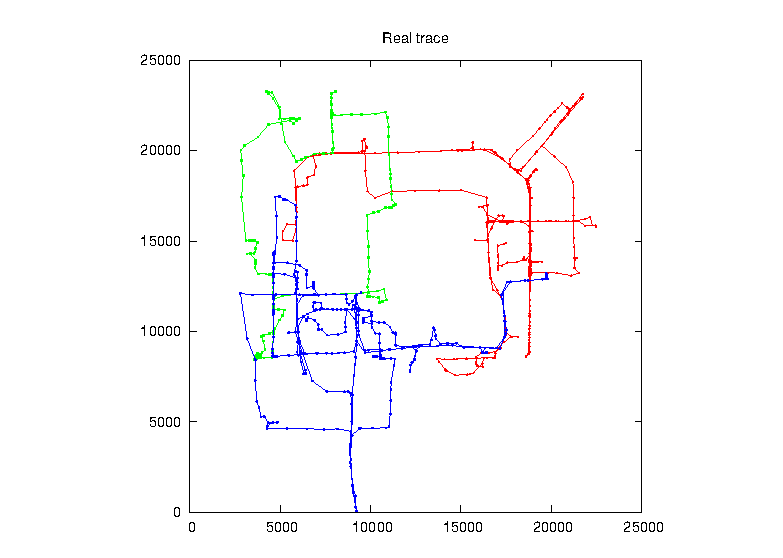
\includegraphics[width=0.23\textwidth]{figures_201103/Evaluation/trace_real.eps}}
%\hspace{0.0in}
%\subfigure[START]{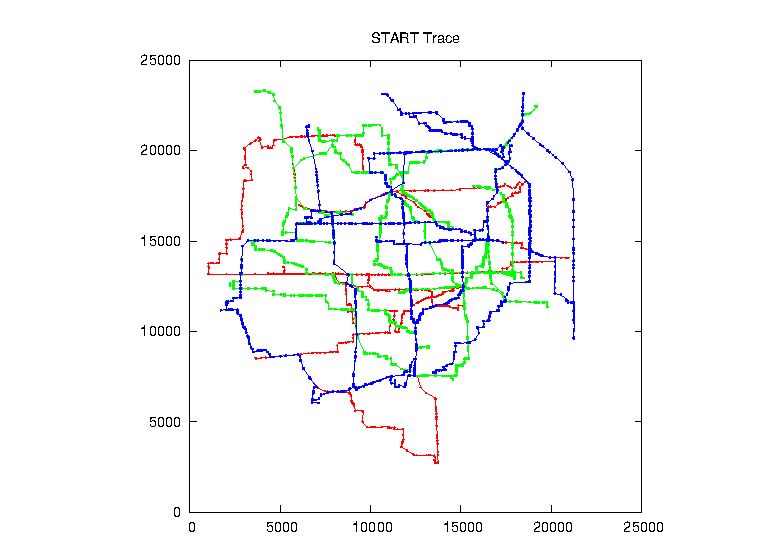
\includegraphics[width=0.23\textwidth]{figures_201103/Evaluation/trace_start.eps}}
%\hspace{0.0in}
%\subfigure[SP]{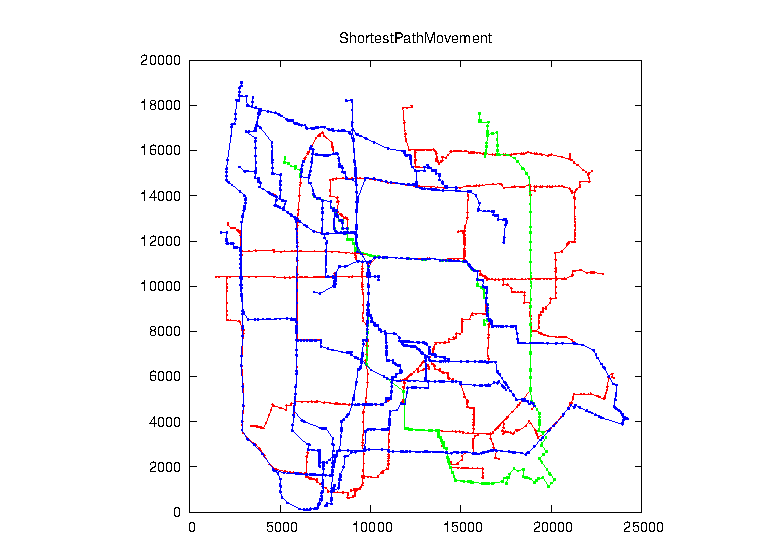
\includegraphics[width=0.23\textwidth]{figures_201103/Evaluation/trace_sp.eps}}
%\hspace{0.in}
%\subfigure[RWP]{\includegraphics[width=0.23\textwidth]{figures_201103/Evaluation/trace_rwp.eps}}
%\caption{Trace samples}\label{figure_tracesample}
%\end{figure}

%\begin{figure}[!h]
%\centering
%\subfigure[Real Trace]{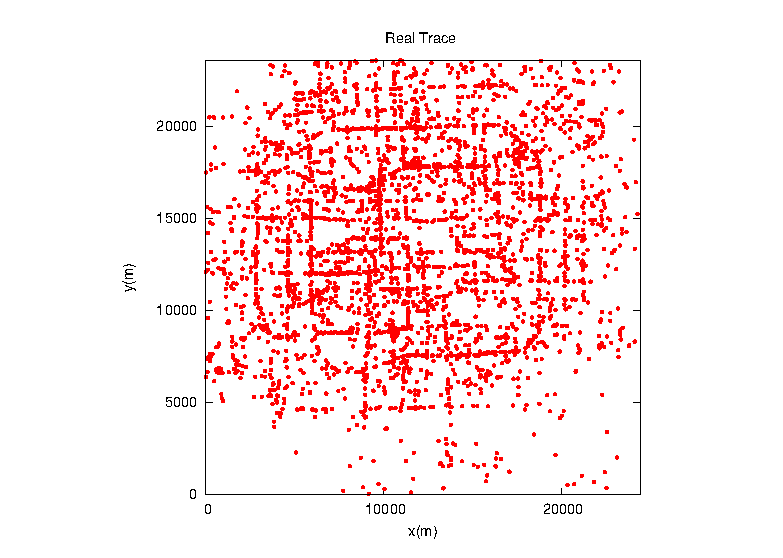
\includegraphics[width=0.23\textwidth]{figures_201103/Evaluation/sample/tracesample.eps}}
%\vspace{0.in}
%\hspace{0.0in}
%\subfigure[START]{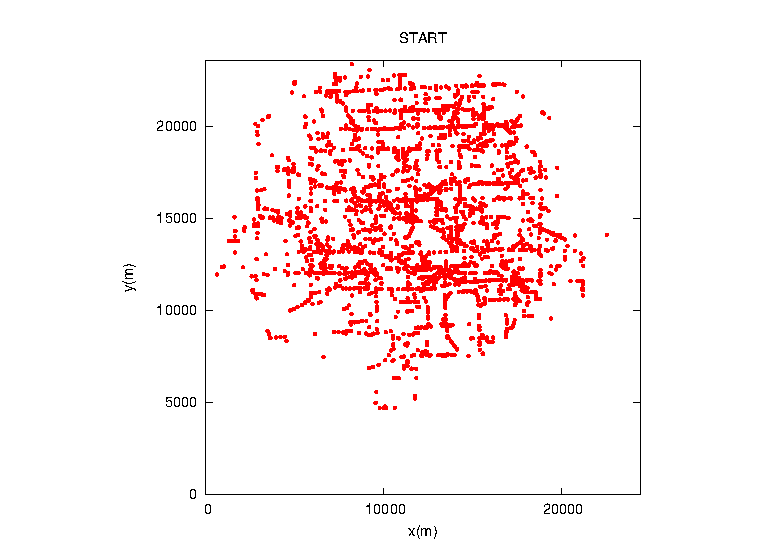
\includegraphics[width=0.23\textwidth]{figures_201103/Evaluation/sample/startsample.eps}}
%\vspace{0.in}
%\hspace{0.0in}
%\subfigure[SP]{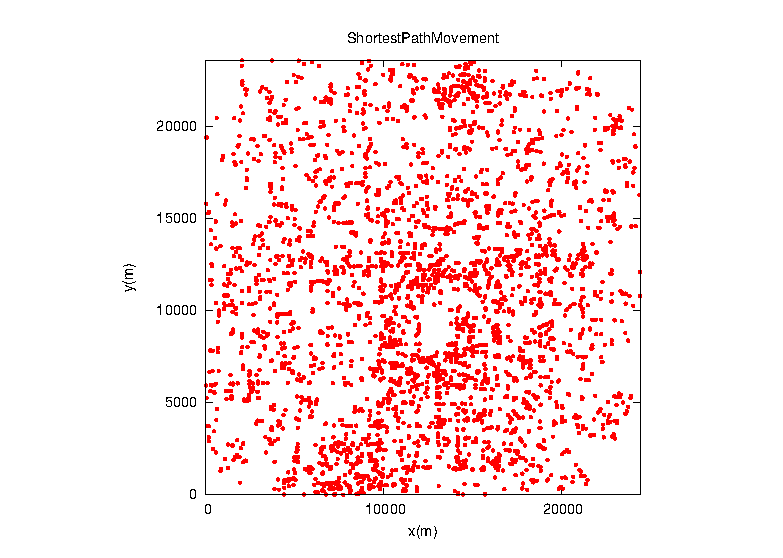
\includegraphics[width=0.23\textwidth]{figures_201103/Evaluation/sample/spsample.eps}}
%\vspace{0.in}
%\hspace{0.0in}
%\subfigure[RWP]{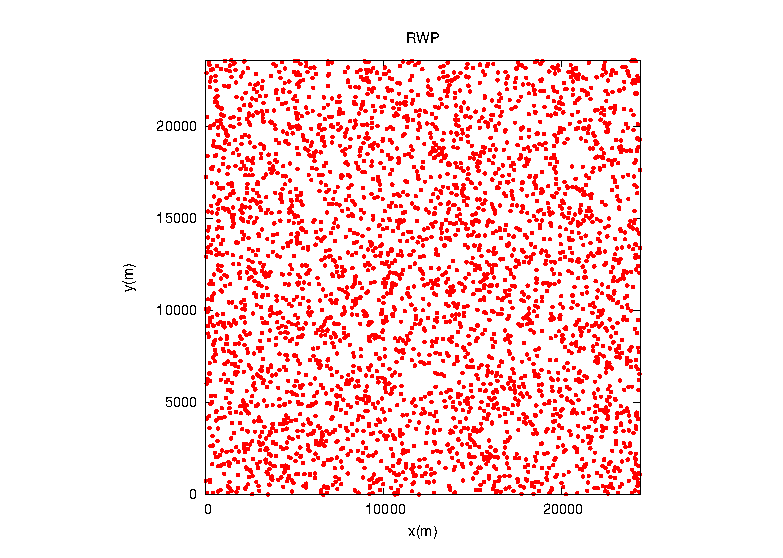
\includegraphics[width=0.23\textwidth]{figures_201103/Evaluation/sample/rwpsample.eps}}
%\caption{Trace snapshots}\label{figure_trace_snapshots}
%\end{figure}

\subsection{Contacts Characteristics}

\begin{figure}[!t]
\centering
\subfigure[cumulative contact time distribution]{
\includegraphics[width=0.35\textwidth]{figures_201103/Evaluation/contact/ct_ccdf.eps}
}
\subfigure[cumulative inter contact time distribution]{
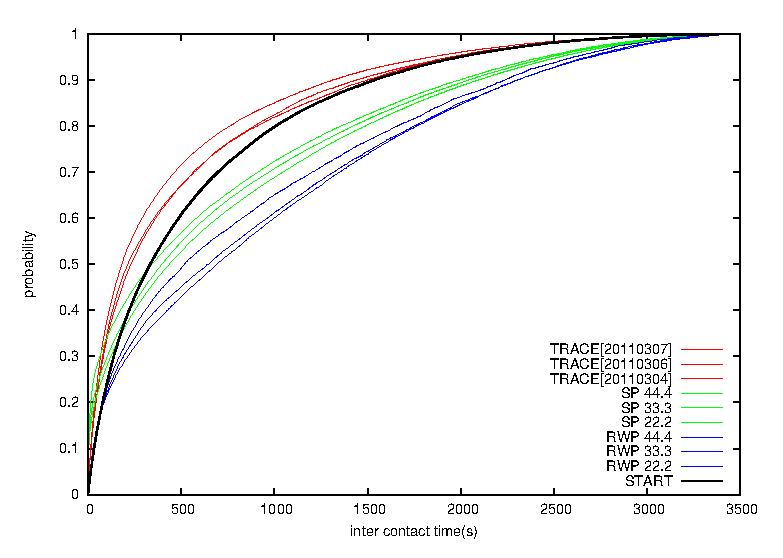
\includegraphics[width=0.35\textwidth]{figures_201103/Evaluation/contact/ict_ccdf.eps}
}
\caption{Contact time, inter contact time distribution.}\label{figure_contacts}
\end{figure}
\begin{figure}[!t]
\centering
\subfigure[time vs. total contact time]{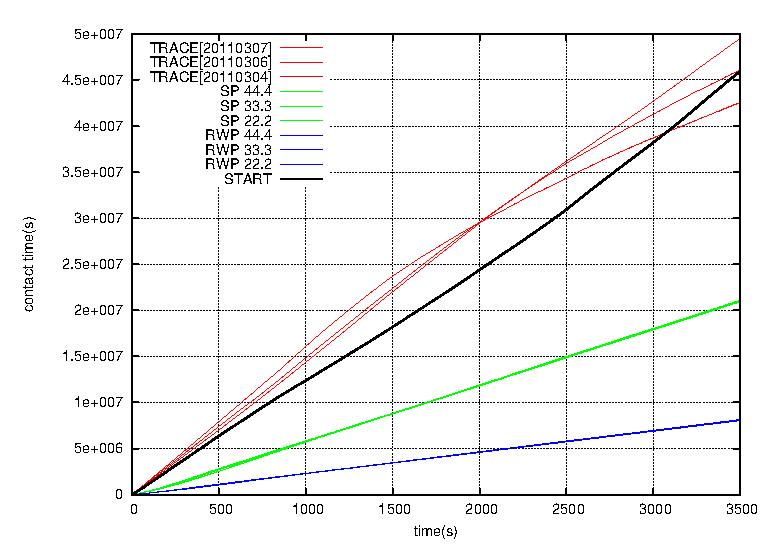
\includegraphics[width=0.38\textwidth]{figures_201103/Evaluation/contact/tc.eps}}
\subfigure[time vs. total contact time in logscale]{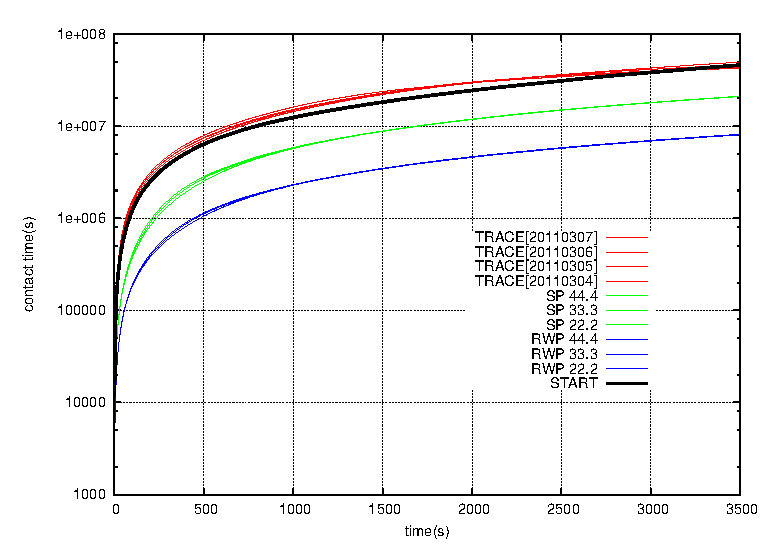
\includegraphics[width=0.38\textwidth]{figures_201103/Evaluation/contact/tc_logscale.eps}}
\caption{Time vs. total contact time.}\label{figure_total_contact_time}
\end{figure}

The contact time and inter contact time among vehicles are also evaluated as the indicators to validate the similarity. 
Fig. \ref{figure_contacts} reports the contact time and inter-contact distributions, which shows the probability of the contact or inter-contact time smaller than certain time length. To substantiate, a point $(25,0.5)$ in the plots means the probability is $0.5$ when contact or inter-contact time is shorter than $25s$. Clearly, START matches the real traces best among three mobility models.
Fig. \ref{figure_total_contact_time} also show the sum of contact time regarding to the simulation time. In Fig. \ref{figure_total_contact_time}(a), the three green lines of SP and the three blue lines of RWP are overlapping with each other. To recognize the differences, we set y axis as log-scale in Fig.~\ref{figure_total_contact_time}(b). The curves of the total contact time vs. time present a liner law. For SP and RWP, the differences of speed ranges show little influence on these curves.
Clearly, the rank of the contact characteristic similarity with the real data is START $>$ SP $>$ RWP.

To conclude, by comparing the node distribution and contact characteristics, the evaluation results confirm that START mobility model achieves great similarities with the real data. START takes the usage of speed and geographic features related with taxi status, while SP employs the map information and RWP is a random model taking use of no realistic data.



\section{Conclusion}
\label{section_conclusion}
Since the mobility model is essential for mobile network, a novel mobility model START based on real GPS trace data is proposed. By assuming the taxi behavior is related with its statuses and geographic feathers, statistical experiments are conducted to verify those assumptions using the real trace data. Further, its parameter--average speed of each status are estimated respectively, and the region transition probability is calculated. In this case, macroscopic movement, a node moves switch between load-event regions and drop-event regions, and microscopic movement(speed for each status) can be defined. Finally, the START is implemented on ONE simulator and estimate it by comparing with the real trace, RWP and Shortest Path mobility Model.
Comparing the node distribution and contact feathers, START shows better performance.
Simulation results demonstrate that START has a good approximation with reality.


\bibliographystyle{IEEEtran}

\bibliography{vehicle_mobility_model}
\appendix

\begin{algorithm}\label{algorithm_connecting}
\caption{Clustering}
\begin{algorithmic}
\STATE \textbf{INPUTs:} $Cells=\{C_{x,y}\}$, the event threshold $\eta$, 
$CLUSTERSCALE$, and $REGION\_ID\_SEED=1$.\\
\STATE $ClusterQueue=\varnothing$ \& $UsedCells=\varnothing$\\
\STATE Sort $Cells$ by events in descending order\\
\FOR{$CELL_{x,y}\in Cells$}
\IF{$CELL_{x,y}\notin UsedCells$}
\STATE¡¡$CELL_{x,y}.region=REGION\_ID\_SEED$\\
\STATE  $size=1$\\
\STATE  $REGION\_ID\_SEED=REGION_ID_SEED+1$\\
\STATE $ClusterQueue.enqueue(CELL_{x,y})$
\STATE $UsedCells.add(CELL_{x,y})$
\WHILE{$ClusterQueue \neq \varnothing$}
\STATE $CELL_{x,y}=ClusterQueue.dequeue()$
\IF{$REGION\_ID\_SEED\leq\_top$ \AND $CELL_{x,y}.events\geq\eta$}
\STATE $enqueueNeighbor(CELL_{x-1,y})$
\STATE $enqueueNeighbor(CELL_{x-1,y-1})$
\STATE $enqueueNeighbor(CELL_{x-1,y+1})$
\STATE $enqueueNeighbor(CELL_{x+1,y})$
\STATE $enqueueNeighbor(CELL_{x+1,y-1})$
\STATE $enqueueNeighbor(CELL_{x+1,y+1})$
\STATE $enqueueNeighbor(CELL_{x,y-1})$
\STATE $enqueueNeighbor(CELL_{x,y+1})$
\ELSE
\STATE $enqueueNeighborOthers(CELL_{x-1,y})$
\STATE $enqueueNeighborOthers(CELL_{x-1,y+1})$
\STATE $enqueueNeighborOthers(CELL_{x-1,y-1})$
\STATE $enqueueNeighborOthers(CELL_{x+1,y})$
\STATE $enqueueNeighborOthers(CELL_{x+1,y-1})$
\STATE $enqueueNeighborOthers(CELL_{x+1,y+1})$
\STATE $enqueueNeighborOthers(CELL_{x,y-1})$
\STATE $enqueueNeighborOthers(CELL_{x,y+1})$
\ENDIF
\ENDWHILE
\ENDIF
\ENDFOR
\end{algorithmic}
\end{algorithm}



\begin{algorithm}
\caption{$enqueueNeighbor(CELL_{x,y})$}
\begin{algorithmic}
\IF{$CELL_{x,y}.events\geq \eta$ \AND $size<clusterSize$ \AND $CELL_{x,y}\notin UsedCells$}
\STATE $ClusterQueue.enqueue(CELL_{x,y})$
\STATE¡¡$CELL_{x,y}.region=REGION\_ID\_SEED$
\STATE $UsedCells.add(CELL_{x,y})$
\STATE $size=size+1$
\ENDIF
\end{algorithmic}
\end{algorithm}

\begin{algorithm}
\caption{$enqueueNeighborOthers(CELL_{x,y})$}
\begin{algorithmic}
\IF{$size<CLUSTERSCALE$\AND $CELL_{x,y}\notin UsedCells$}
\STATE $ClusterQueue.enqueue(CELL_{x,y})$
\STATE¡¡$CELL_{x,y}.region=REGION\_ID\_SEED$\\
\STATE $UsedCells.add(CELL_{x,y})$
\STATE $size=size+1$
\ENDIF
\end{algorithmic}
\end{algorithm}

\end{document}
\endinput




